\documentclass[12pt]{article}% Language setting
\usepackage[english]{babel}

% Page size and margins
\usepackage[letterpaper,top=2cm,bottom=2cm,left=3cm,right=3cm,marginparwidth=1.75cm]{geometry}

% Useful packages
\usepackage{amsmath}
\usepackage{graphicx}
\usepackage{setspace}
\usepackage[colorlinks=true, allcolors=blue]{hyperref}
\usepackage{natbib}
\usepackage{verbatim}
\usepackage{graphicx}
\usepackage{longtable}
\usepackage{array}
\usepackage{hyperref}

\bibliographystyle{plain}

\title{From Bottlenecks to Breakthroughs: A Year Building Assessment Tools for Reliability and AI\\
\large Building Secure, Scalable, and Data-Driven Assessment Systems}
\author{Adam A. Bramlett\\
Graduate Assessment Fellow, Dietrich College of Humanities and Social Sciences }

\begin{document}
\doublespacing
\maketitle

\begin{abstract}
This document details the development of a transformative suite of assessment tools created over the 2024-25 academic year through the Graduate Assessment Fellowship for the Dietrich College General Education Program. Addressing longstanding bottlenecks in educational evaluation, the work spans three integrated projects: (1) a dynamic rating application that standardizes and streamlines the scoring of student artifacts, (2) a flexible reliability script designed not only to assess human inter-rater agreement but also to support rigorous evaluation of AI-generated outputs, and (3) an AI-assisted content generation workflow that accelerates the artifact rating while attempting to maintain pedagogical rigor. Together, these tools establish a scalable, data-driven infrastructure for modern assessment practices, positioning Dietrich College at the forefront of responsible innovation in both human and AI-assisted evaluation.
\end{abstract}

\section{Introduction}

The growing complexity and scale of educational assessment necessitates tools that are efficient, reliable, and adaptable \cite{pellegrino2001k, holmes2021AI}. As part of the Graduate Assessment Fellowship at Dietrich College, a suite of projects was undertaken to address key bottlenecks in the assessment cycle. These projects span the rating, reliability, and content generation phases of assessment work, collectively building a more robust infrastructure for evaluating student learning outcomes.

\section{Rating Application for Scoring}

The first major project involved the development of a comprehensive, dynamic rating application using R and the Shiny framework. The goal was to create an intuitive, efficient environment for data raters to complete assessment scoring tasks, while ensuring data consistency, user security, and minimizing administrative overhead.

Prior to the creation of the app, the rating process was extremely cumbersome. Raters were required to manually look up assignment prompts, locate the appropriate rubrics, and match these to individual student artifacts, often working across multiple documents without any integrated guidance. Given the sheer number of courses, assignments (ranging from 1-5 per course), and artifacts (ranging from 1-60+ per assignment), this process was both time-consuming and had the potentional to be more error-prone (caused primarily by the comoplexity of the task). Artifacts, here, refers to individual assignments of work completed by the students. It was especially challenging on standard computer screens, where managing numerous files and windows simultaneously made the workflow nearly impossible. There was no built-in way to ensure that the correct instructions and rubrics corresponded to the artifacts being scored, leading to confusion, inconsistencies in scoring, and inefficiencies across the entire assessment process. Figure~\ref{fig:rating_app} shows a comparison of how the previous rating task was done before the app and how it appears to the user for comparison. 

\begin{figure}[!h]
    \centering
    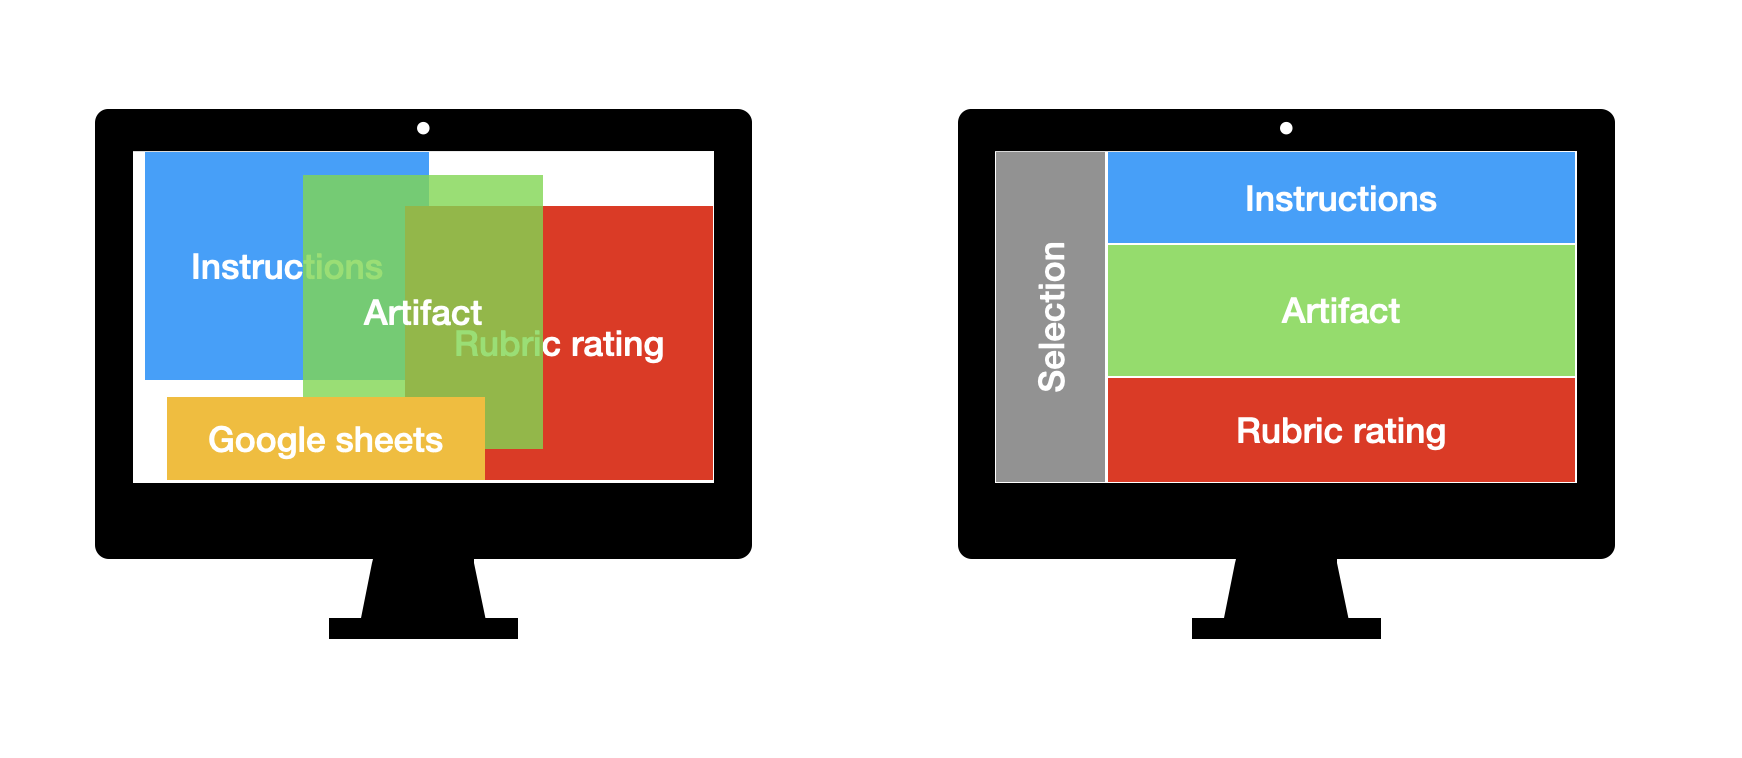
\includegraphics[width=1\textwidth]{visualizations/rating_app.png}
    \caption{Rating App: Left side shows the prior workflow for rating individual artifacts. The right shows the customized app for submitting ratings. Notice that the workflow is now cleanly delineated and removes the need for an extra window for recording artifact ratings as this is built into the structure. A selection tool keeps moving through artifacts fast and efficient.}
    \label{fig:rating_app}
\end{figure}

Security was also a critical challenge in the pre-existing system. Student artifacts often contained sensitive or personally identifiable information, systematic controls were in place yes limited to restrict access. However, artifacts were often unnecessarily downloaded to manage them for individual raters. To address this, the new application incorporates a secure login system, requiring raters to authenticate before accessing any assignment materials or rating interfaces. Figure~\ref{fig:password_gaf_app} shows the password-gated login screen implemented to ensure that only authorized users could interact with student artifacts and scoring data. This stage was a crucial step that allows clear tracking of ratings but also retains the privacy necessary for protecting the content of the artifacts.

\begin{figure}[h]
    \centering
    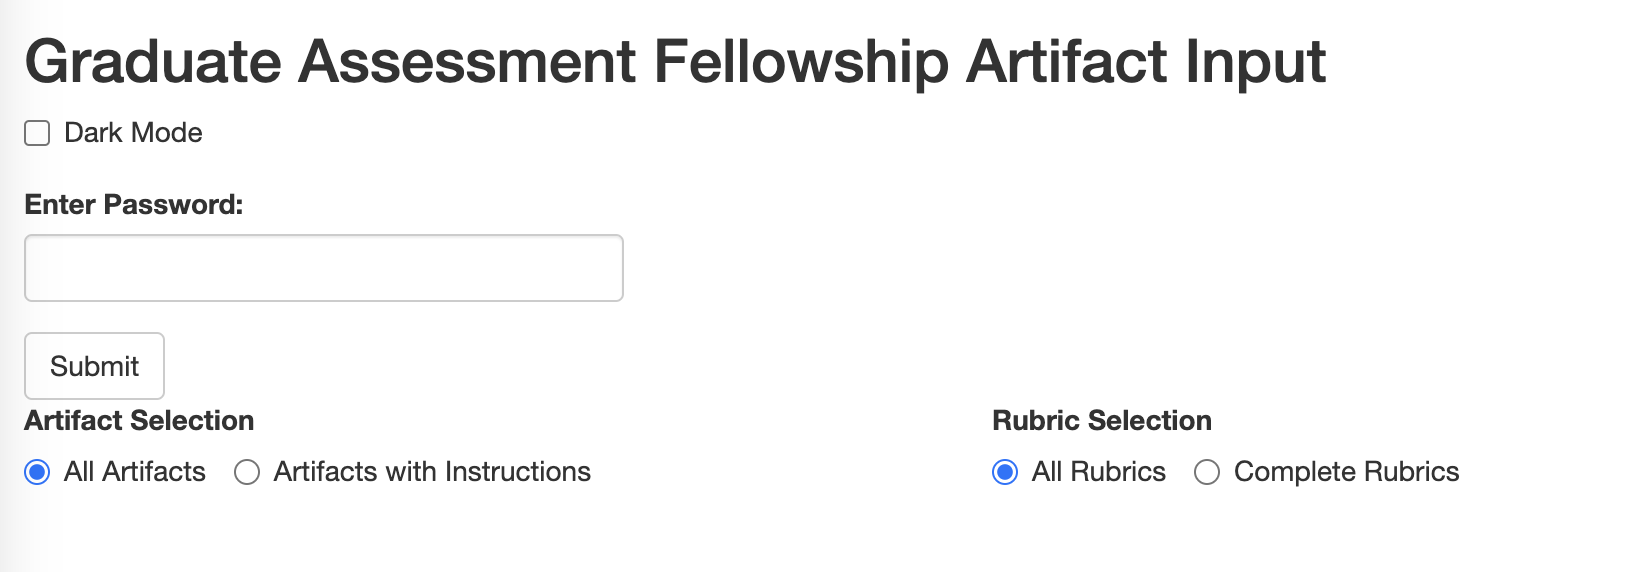
\includegraphics[width=1\textwidth]{visualizations/password_gaf_app.png}
    \caption{Login screen for the GAF rating application.}
    \label{fig:password_gaf_app}
\end{figure}

Beyond security improvements, the new application fundamentally solved the workflow problems by consolidating the entire rating process into a single, responsive interface. Raters can now select the Learning Outcome area (e.g., Intercultural \& Global Inquiry, Interdisciplinary Perspectives, etc.), Course, Semester, Assignment, and Student Artifact through a series of cascading dropdown menus. See "Selection" on the right side of Figure  \ref{fig:rating_app}. Each selection dynamically filters the available options for the next, ensuring that raters are only presented with valid and context-appropriate choices. Once an artifact is selected, the corresponding assignment prompt and full rubric are automatically retrieved and displayed within the app. This integration eliminates the need for manual cross-referencing and ensures that raters always have the exact information they need directly in front of them.

Figure~\ref{fig:sample_instructions_artifact_example} illustrates the interface where raters are presented with the assignment instructions alongside the student artifact, enabling them to score submissions with full context.

\begin{figure}[h]
    \centering
    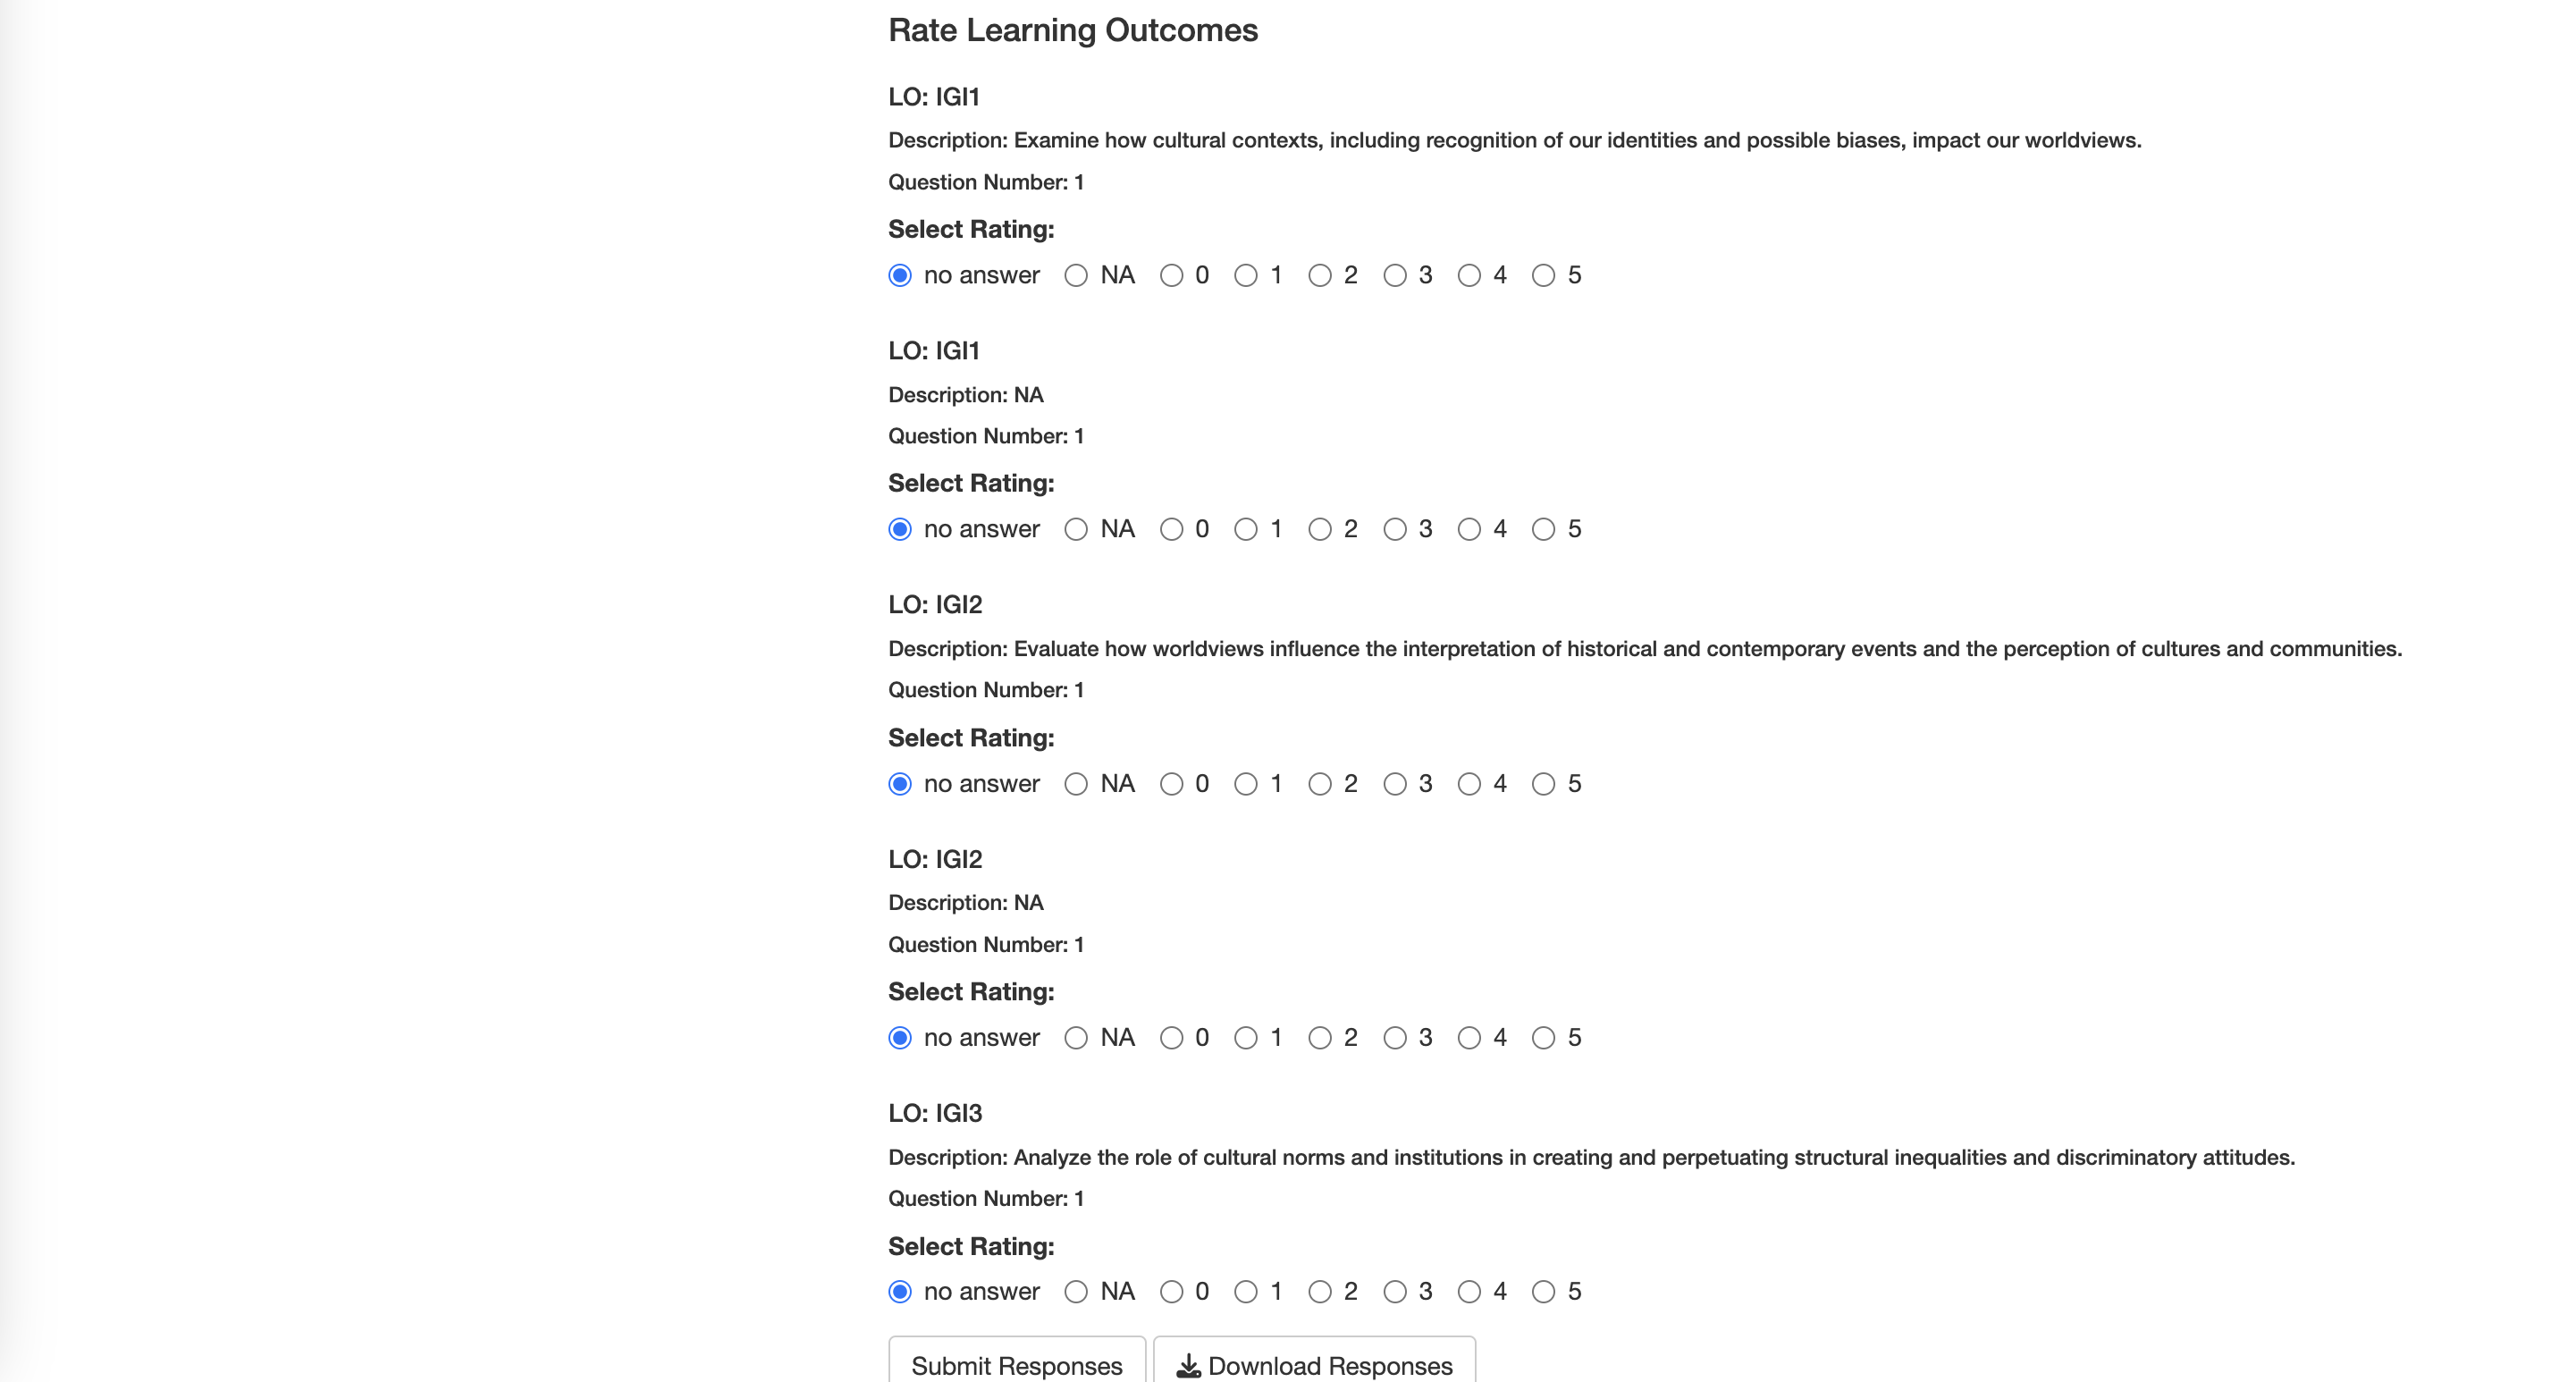
\includegraphics[width=1\textwidth]{visualizations/sample_instructions_artifact_example.png}
    \caption{Display of assignment instructions and sample student artifact during rating.}
    \label{fig:sample_instructions_artifact_example}
\end{figure}

The rating interface itself was carefully designed to be both interactive and intuitive. Raters assign scores to each rubric row through dynamically generated input fields, and text boxes are provided for entering qualitative feedback when appropriate. Figure~\ref{fig:rubric_scoring} shows an example of the rubric scoring interface. To preserve data quality, the app enforces a validation check: users cannot submit their ratings unless all rubric rows have been completed, with clear feedback provided if any entries are missing. Raters also have the flexibility to skip an artifact if necessary or return to the home screen to select a different assignment, accommodating a range of practical needs during large-scale scoring projects.

\begin{figure}[h]
    \centering
    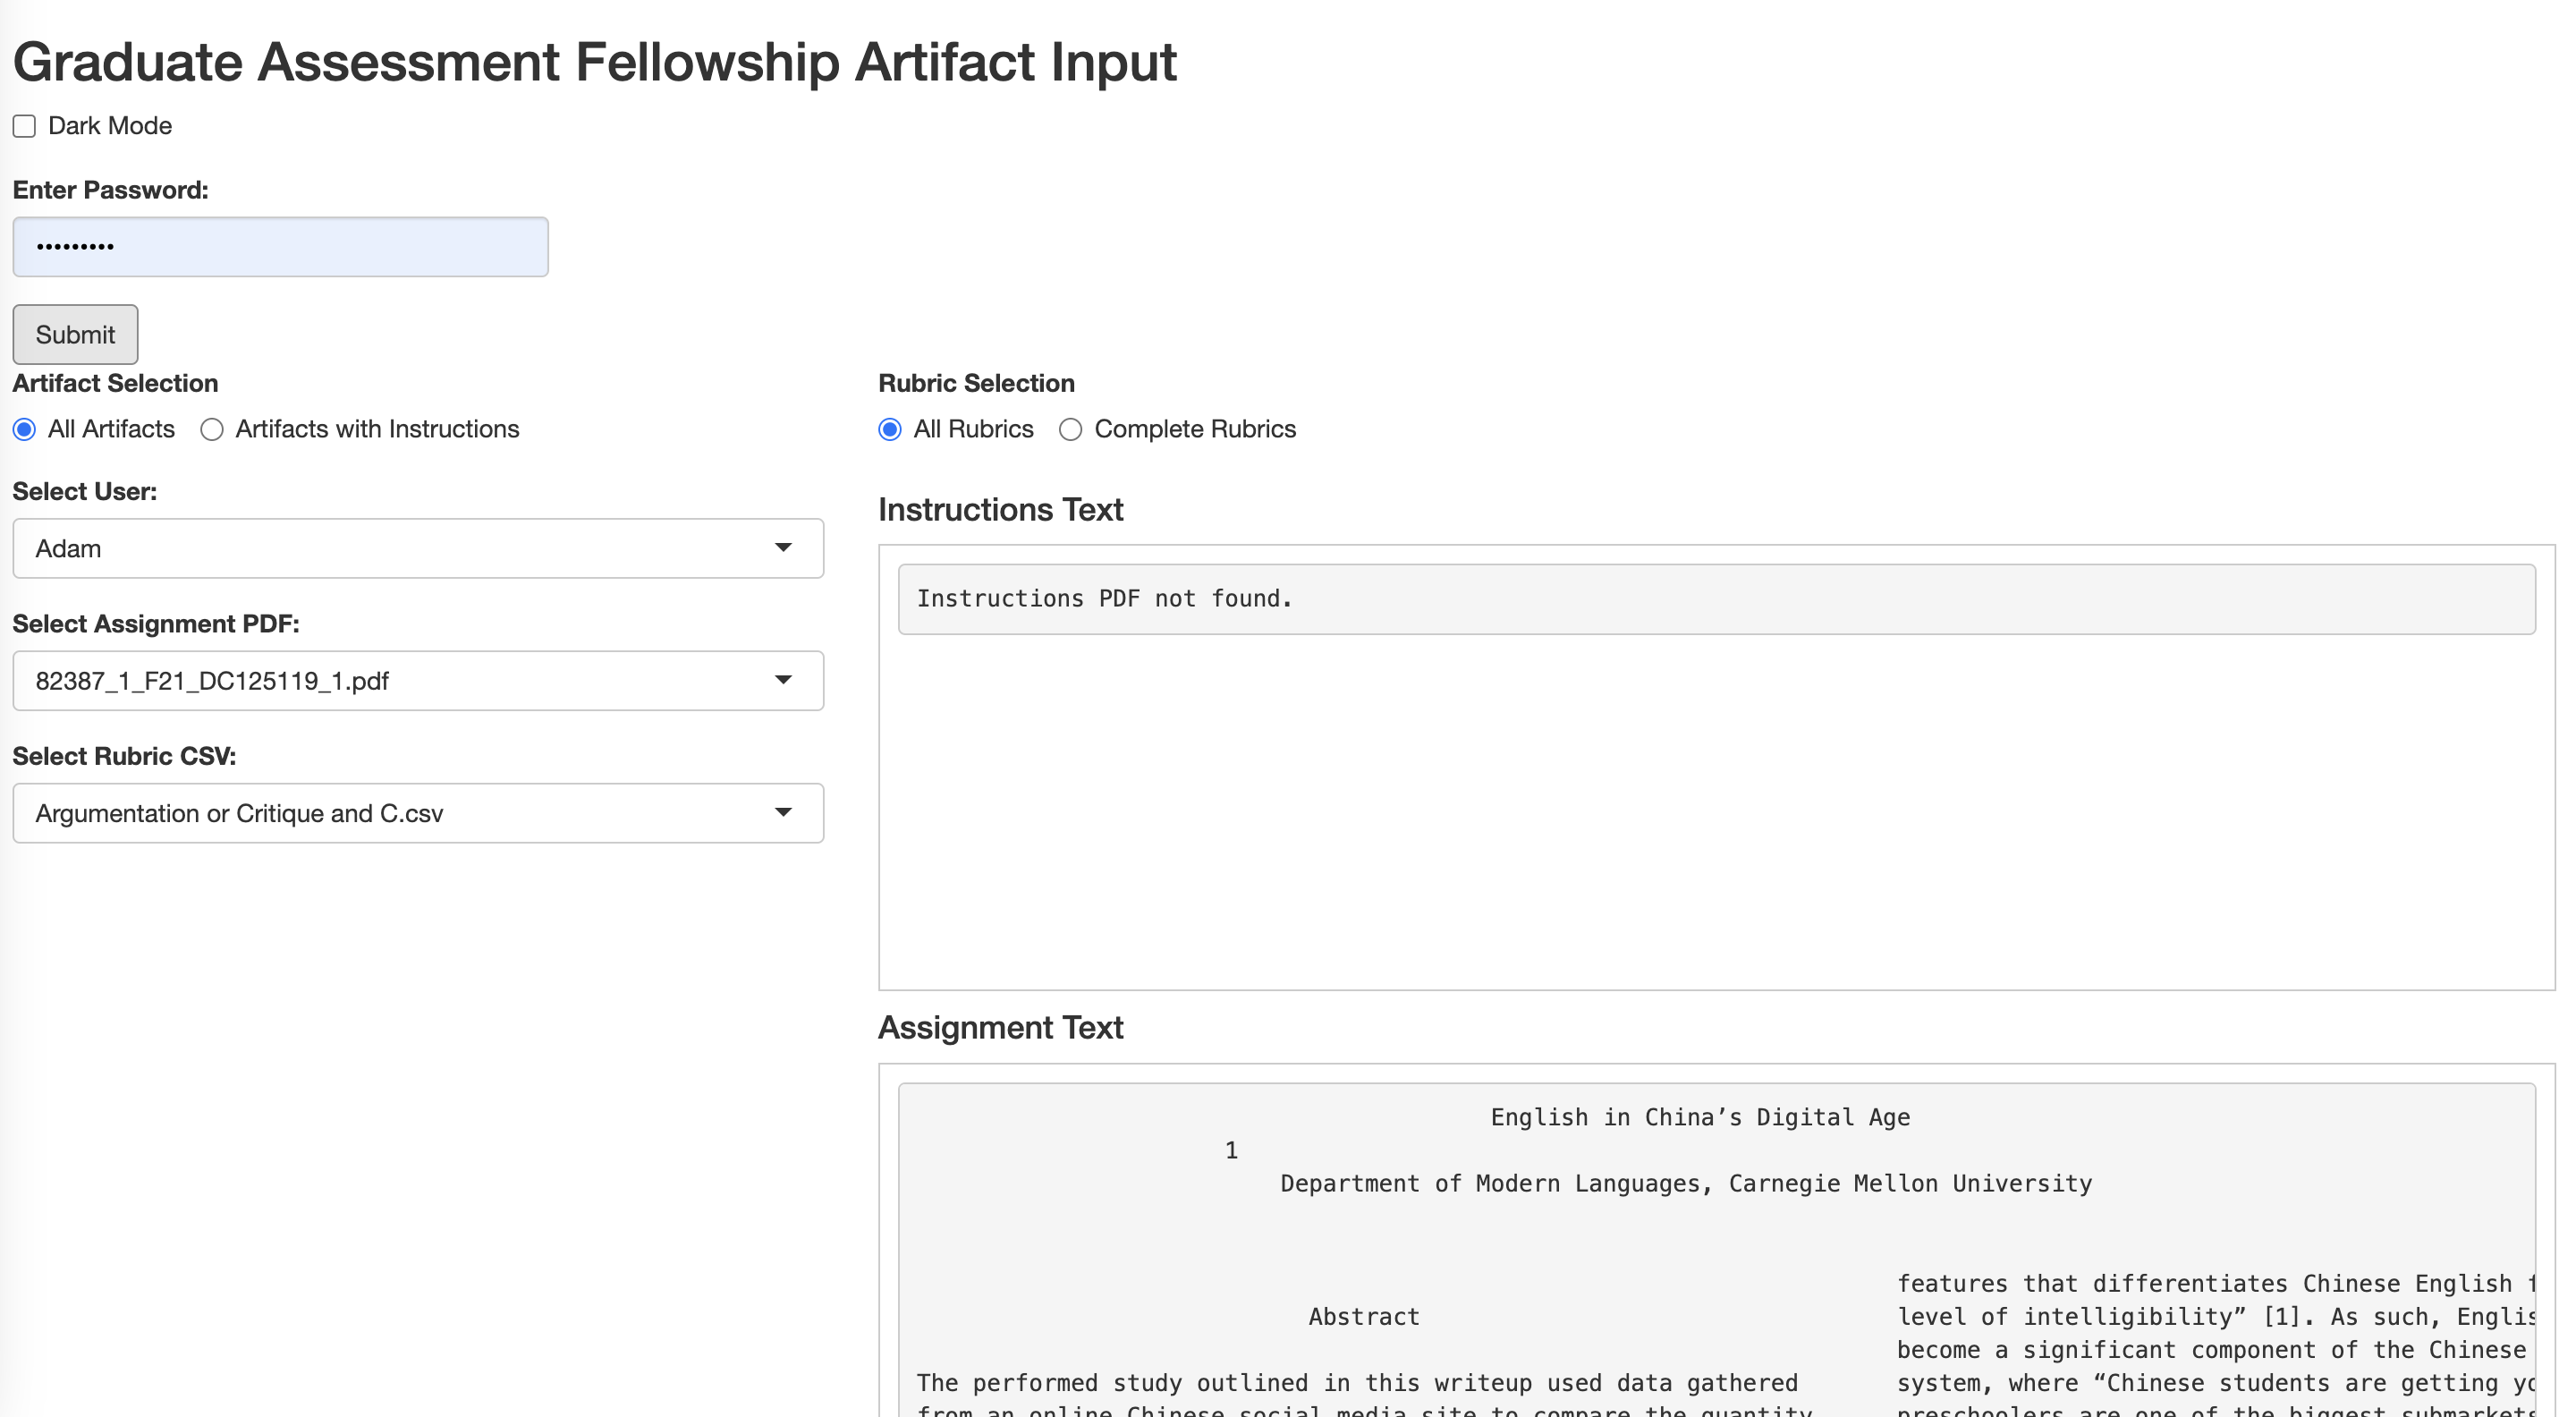
\includegraphics[width=0.45\textwidth]{visualizations/rubric_scoring.png}
    \caption{Interface for rubric-based scoring within the rating application.}
    \label{fig:rubric_scoring}
\end{figure}

Behind the scenes, all ratings are automatically saved into organized google sheets files, with naming structures tied systematically to assignment and artifact identifiers. Data storage was intentionally designed to follow tidy data principles, allowing easy aggregation and analysis of ratings for reliability studies and reporting. Figure~\ref{fig:tidy_data_stored_example} shows an example of the structured output generated by the system after ratings are submitted.

\begin{figure*}[h]
    \centering
    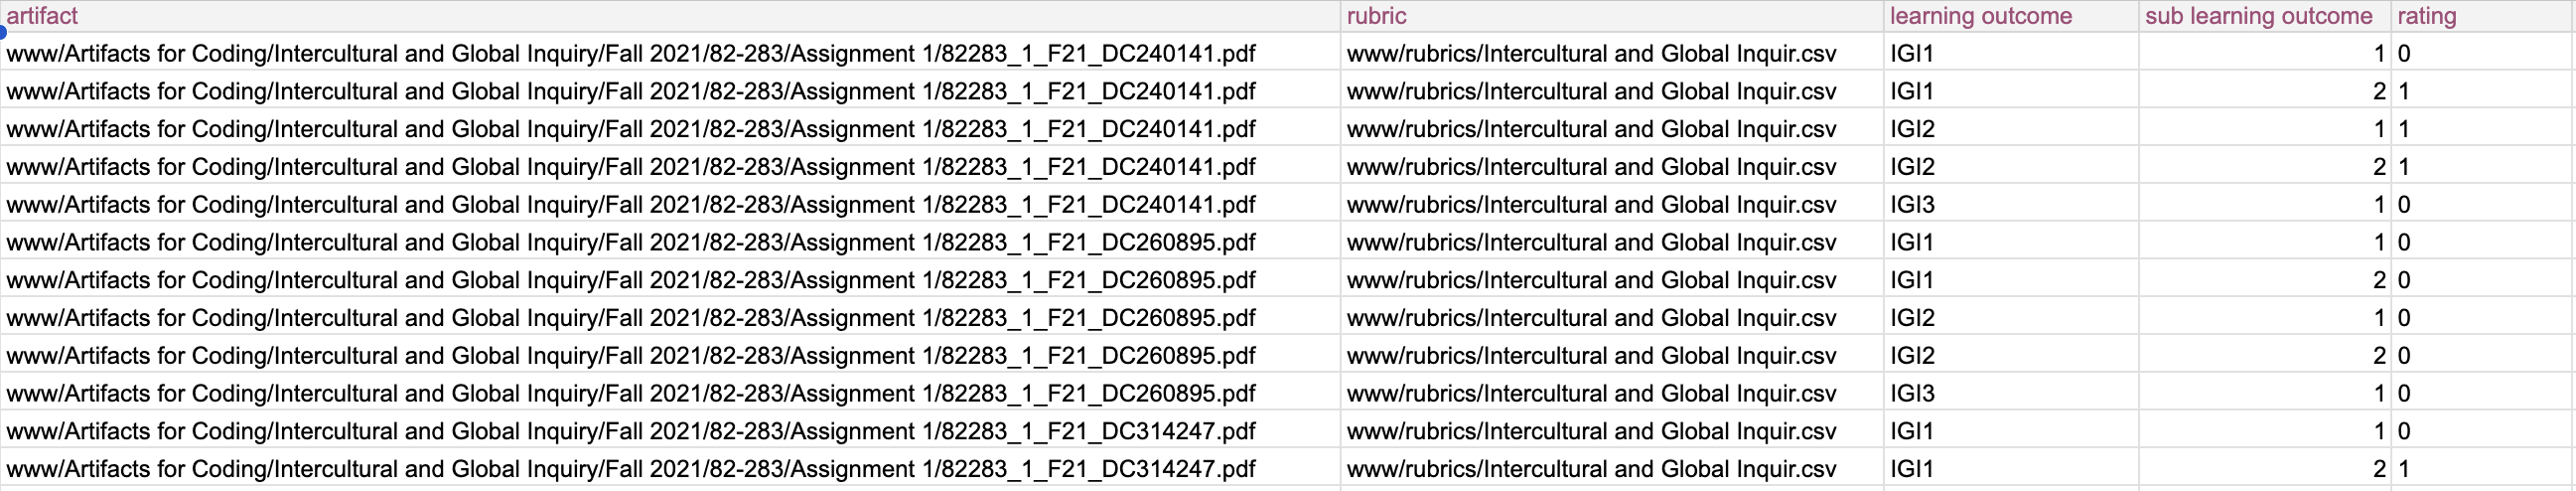
\includegraphics[width=1\textwidth]{visualizations/tidy_data_stored_example.png}
    \caption{Example of structured, tidy data storage from rating submissions.}
    \label{fig:tidy_data_stored_example}
\end{figure*}

The application's codebase was structured with future extensibility in mind. Interface elements such as the rubric display and prompt loading were modularized into reusable functions (e.g., \texttt{generateRubricUI}, \texttt{generatePromptUI}), making it easy to adapt the system for future assessment types, expanded rubric formats, or evolving security requirements. This design choice ensures that the rating platform remains sustainable and scalable as assessment needs grow.

By addressing the significant bottlenecks of the previous manual system —both operational and security-related— this dynamic rating application not only reduces administrative burden but also enhances accuracy, standardization, data protection, and user experience. It establishes a scalable, future-proof framework that can easily support broader assessment initiatives across Dietrich College and beyond.

The central goal of this artifact scoring app was to create a dynamic rating application, built with R and Shiny, that replaced a cumbersome, manual scoring process with a secure, user-friendly interface. This new system allows raters to access assignment prompts, rubrics, and student artifacts in a single view, dramatically improving workflow efficiency, scoring accuracy, and data security. Features include cascading selection menus, real-time validation, and structured, tidy data storage for analysis. The application was designed to be modular and extensible, ensuring adaptability for future needs. \textbf{This effort marks a shift toward scalable, data-driven assessment and supports both human and AI-assisted evaluation systems.}

\subsection*{Reliability Project and Test Case}

Reliability is foundational to any assessment endeavor. Without strong inter-rater reliability, scores assigned to student artifacts risk being inconsistent, biased, or arbitrary, undermining both the credibility of the assessment system and the fairness extended to students. In traditional human scoring contexts (for example SAT writing and/or test grading), even trained raters can diverge in their interpretations of rubric criteria, inferences about student intent, or judgments about partial credit. 

The introduction of AI-generated scoring presents a parallel but distinct set of challenges. While AI models like ChatGPT offer impressive linguistic fluency and efficiency, they are not immune to inconsistency or bias, particularly when working with complex, discipline-specific rubrics \citep{atasoy2025}. Evaluating AI reliability is therefore not a mere formality; it is a necessary empirical check to ensure that automation enhances, rather than compromises, the integrity of educational assessment.

\section{Reliability Script for Inter-Rater Agreement}

The second major project focused on the creation of a robust R Markdown script for evaluating inter-rater reliability. This tool was developed to serve a dual purpose: first, to assess the consistency and validity of human rater judgments, and second, to lay the groundwork for future comparisons between human ratings and AI-generated outputs. As the Dietrich College General Education Program increasingly explores the use of \href{https://studentprivacy.ed.gov/ferpa}{AI tools} to assist in assessment tasks, it is crucial to have a rigorous, transparent method for quantifying how closely AI-generated ratings align with human standards.

The reliability script intelligently merges datasets from multiple raters based on shared artifact identifiers, ensuring that scores for the same assignment submissions are accurately paired. The script offers flexible column matching, allowing users to specify which rubric rows or metrics they wish to check for agreement. It calculates multiple measures of reliability, including exact percent agreement (the proportion of identical ratings across raters) \cite{gwet2014}, one-off agreement (the proportion of ratings that are within a one-point difference), and Cohen's Kappa (a chance-corrected measure of agreement) \cite{cohen1960, mchugh2012} for each rubric row individually. This multi-metric approach provides a more nuanced understanding of scoring consistency across different levels of granularity.

Special attention was given to handling missing data and inconsistencies. The script identifies and filters out artifacts with missing or skipped ratings, ensuring that reliability metrics are based only on comparable entries and are not artificially inflated or deflated. The outputs of the script include clean, interpretable summary tables that display reliability results by rubric row, artifact, and overall scoring dimensions. These tables are formatted for easy interpretation and direct inclusion in assessment reports or internal documentation.

The reliability script was also designed with extensibility in mind. New rubric rows, additional rater datasets, or alternative agreement metrics can be incorporated with minimal adjustment. This flexibility ensures that the tool remains sustainable as assessment practices evolve, including its planned use in evaluating the performance of AI models. As such, it plays a critical role not only in current reliability checks but also in positioning the Dietrich College to make informed decisions about integrating AI into the assessment process.
This reliability script allows assessment teams to quickly identify strengths and weaknesses in rater calibration and to provide targeted feedback for training.

\begin{figure}[h]
    \centering
    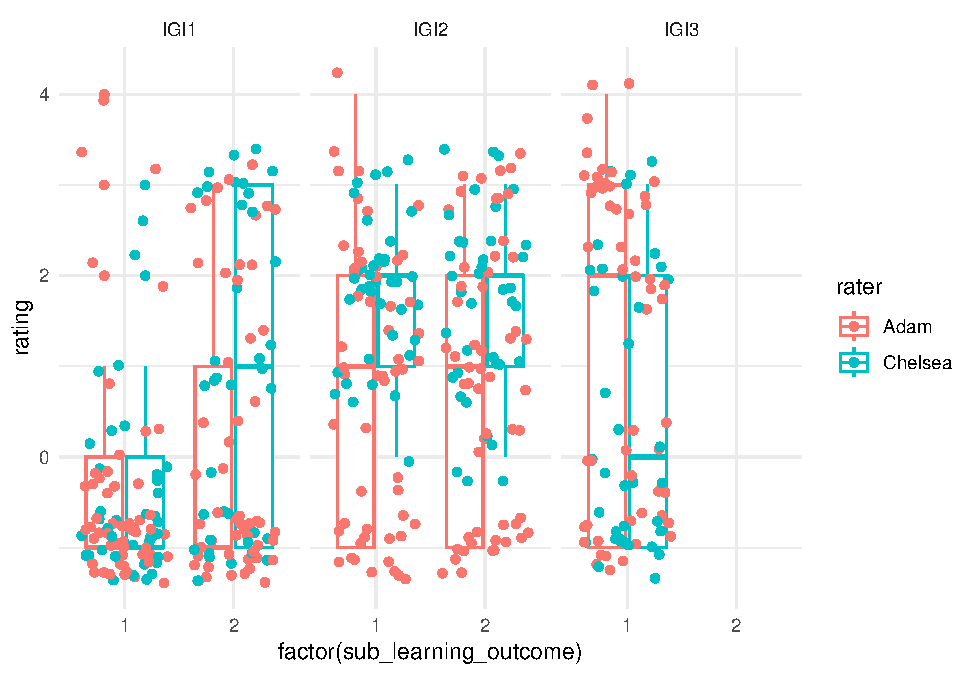
\includegraphics[width=1.0\textwidth]{visualizations/unnamed-chunk-3-1.pdf}
    \caption{Example reliability output generated during rater and model evaluation.}
    \label{fig:reliability_output}
\end{figure}

\subsection*{Reliability Script for Inter-Rater Agreement and AI Model Evaluation}

A central goal of assessment of the Dietrich College General Education Program is to ensure that scoring practices are consistent, valid, and reflective of student achievement across a diverse range of assignments, disciplines, and learning outcomes. In support of this mission, one of the major projects completed during the fellowship year was the development of a comprehensive R Markdown script designed to evaluate inter-rater reliability. However, the purpose of this tool extends beyond traditional human-human agreement checks. It was also architected to support the systematic evaluation of AI model outputs, particularly as large language models like ChatGPT are increasingly considered for use in educational assessment. As such, the reliability script stands as a crucial infrastructure component, linking traditional assessment practices to emerging AI-based innovations.

While the pipeline for reliability has been created to be able to test reliability on any of the artifacts or select rubrics, this year, we have chosen to focus on the Intercultural and Global Inquiry (IGI) rubric as a starting point. The reasoning behind this was three fold: 1) convenience, completion, and AI extendability. Many rubrics have already been made for the graduate assessment fellows over past years. However, the reliability of these rubrics is unknown. We chose IGI because of how many clear samples there were so that we could test our own reliability in a known case. Secondly, IGI has limited artifacts that follow a generally similar assignment structure. That is, the assignments are straightforward and are limited in type (e.g., all written assignments like essays). This is not to indicate that limited assignment type is a good thing in general but for reliability testing it is ideal. Such assignments are ideal for testing reliability. Lastly, because our goal was to have these artifacts rated by AI, we needed to choose an artifact group that had enough for testing variation. In this way, we can see the selection of IGI as an ideal test case for both tests of reliability and for AI extensions.

\subsubsection*{IGI as a Test Case for Reliability Evaluation}

To assess how well the reliability pipeline performs under real-world constraints, we applied it to a subset of artifacts drawn from the Intercultural and Global Inquiry (IGI) area. IGI was chosen for three reasons: its well-structured assignment types, the availability of samples from Fall 2021 to Fall 2024, and its suitability for AI extension. Unlike some other domains where assignments vary dramatically in scope or genre, IGI artifacts tend to share a relatively uniform format. This made it possible to isolate variation due to rater behavior or rubric interpretation, rather than confounding it with uncontrolled differences in assignment design. Additionally, a large number of artifacts in this area had already been scored in past assessment cycles, providing a baseline for comparison. Finally, IGI aligns well with the kinds of reflective, multi-criteria evaluation tasks that large language models are increasingly being used to support, making it a natural testbed for human-AI comparisons \cite{li2025, wang2025}.

Using this dataset, we tracked the reliability of two human raters over time as they evaluated IGI artifacts using the \href{https://docs.google.com/spreadsheets/d/1LFFnQgPI8yS5Dcm3NNLW2Vmmojya27OXNudUB8O3ja0/edit?gid=890635860#gid=890635860}{official rubric}. The aim was to understand not only whether rater agreement improved with practice, but also whether certain rubric rows or criteria consistently posed more difficulty than others. This analysis allowed us to identify patterns in scoring behavior and to determine whether rubric components converged toward acceptable levels of reliability (typically defined as Cronbach’s alpha values above .6 or .7 \cite{cronbachalpha}). In other words, we were not only interested in whether raters agreed overall, but whether that agreement held across the full structure of the rubric.

Throughout this document, rubric subcomponents are referenced using both numeric (e.g., 2.1, 2.2) and lettered (e.g., 2a, 2b) labels. This dual system was adopted to serve two audiences: faculty across Dietrich College and future students fellows in the Graduate Assessment Fellowship. Our goal was to strike a balance between transparency and long-term usability. While rubric components such as IGI2.1 and IGI2a refer to the same construct---evaluation of how worldviews influence interpretation of events---we opted to retain the numeric labeling (e.g., 2.2) in the \texttt{R} codebase and visual outputs. This choice simplifies downstream processing and ensures consistency across automated workflows. At the same time, we preserved cross-references to the original rubric structure to maintain clarity for faculty reviewers. This dual-labeling approach supports both immediate interpretability and future extensibility.

\subsection*{Multi-Level Reliability Tracking}

The IGI rubric contains three broad learning outcomes, each of which is subdivided into additional fine-grained criteria. For instance, IGI1 focuses on self-reflection and the recognition of cultural context in shaping personal and others’ worldviews, while IGI2 centers on how those worldviews influence interpretation and perception of social and historical events. IGI3 targets analysis of structural inequality and cultural institutions. Each of these outcomes is represented by multiple rubric rows, and many of those rows themselves contain subcomponents — such as personal vs. others’ worldviews, or event interpretation vs. community perception — that require distinct evaluative judgments.

To capture this layered structure, our reliability analysis proceeded at three levels. First, we computed an overall reliability score for each batch of rated artifacts, tracking whether general rater agreement increased across rating sessions. Second, we broke this down by primary learning outcome — IGI1, IGI2, and IGI3 — to detect whether any outcome posed more consistent scoring challenges than others. Third, we examined reliability within the sub-categories (e.g., IGI1a, IGI1b, etc.) of each rubric outcome, identifying exactly where scoring drift, misunderstanding, or inconsistency occurred.

This multi-level approach provides a more precise view of where reliability breaks down, allowing for targeted interventions in rubric training or clarification. For example, if rater agreement is high for IGI1 overall but low for the subcomponent related to others’ worldviews (IGI1b/IGI1.2), we know where to direct future calibration efforts. By tracking how each of these dimensions changes over time, we can also measure the effectiveness of training and experience, distinguishing temporary variation from systemic issues in the rubric itself. These results offer the most detailed picture to date of how rubric design, rater interpretation, and artifact variation interact in practice — and form the basis for future AI-human comparison studies in assessment reliability.


\subsection*{Data Analysis}

In our first analysis, we used Cronbach’s alpha \cite{cronbachalpha} to track changes in inter-rater reliability over time for the IGI artifact set. Figure~\ref{fig:overal_reliability} presents an overall measure of reliability across rated item, capturing whether the two primary raters showed increased agreement as they progressed through the task. 53 artifacts were rated in total. The results suggest a modest upward trend, with alpha scores approaching the conventional threshold for acceptable reliability. Although early sessions showed lower internal consistency, subsequent batches stabilized, suggesting that the raters became more calibrated through experience, discussion, or increased familiarity with the rubric.

\begin{figure}[h]
    \centering
    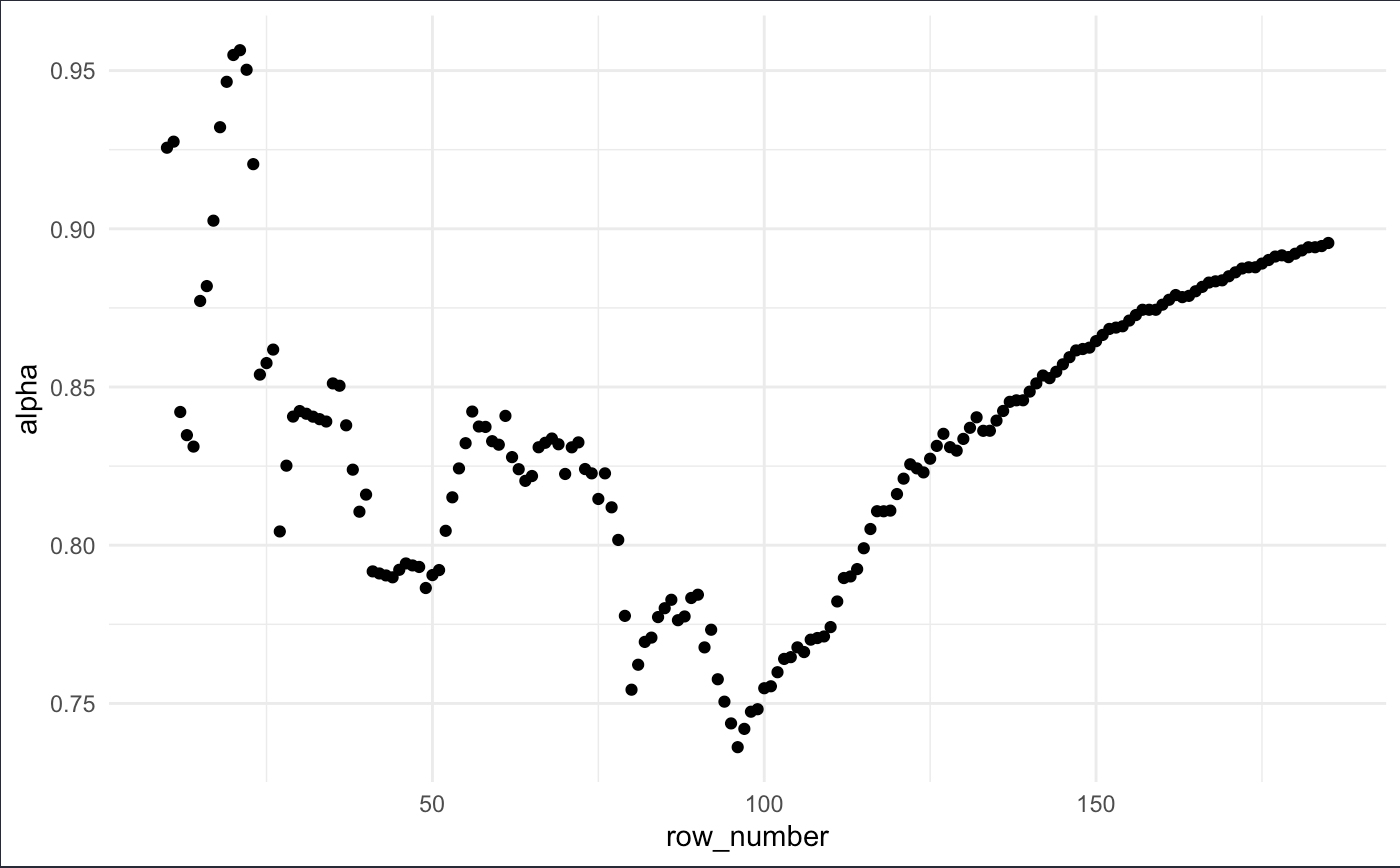
\includegraphics[width=1.0\textwidth]{visualizations/overal_reliability.png}
    \caption{This visual shows reliability over time between two raters using the same rubric on the same assignments. The rating reliability is much more variable at the beginning. However, over time after rating approximately 100 sub-rubric scorings, the rating appears to have a steady increase and asymptotes to .9 reliability, which is extremely high.}
    \label{fig:overal_reliability}
\end{figure}


To better understand where this improvement was coming from —and whether some parts of the rubric were contributing more to overall reliability than others— we broke down the analysis by the three primary learning outcomes: IGI1, IGI2, and IGI3. This analysis, shown in Figure~\ref{fig:sub_sect_reliability}, revealed some divergence in how reliably each outcome was scored. IGI1, which emphasizes reflective writing about personal and others’ worldviews, consistently showed the highest reliability across batches. IGI2, focused on evaluating how worldviews influence interpretation, showed more variability, particularly in early batches. IGI3, which targets structural inequality and institutional analysis, presented the most inconsistency. This may be due to the broader interpretive range of responses that this outcome elicits, or potentially to how its rubric is phrased.

\begin{figure}[h]
    \centering
    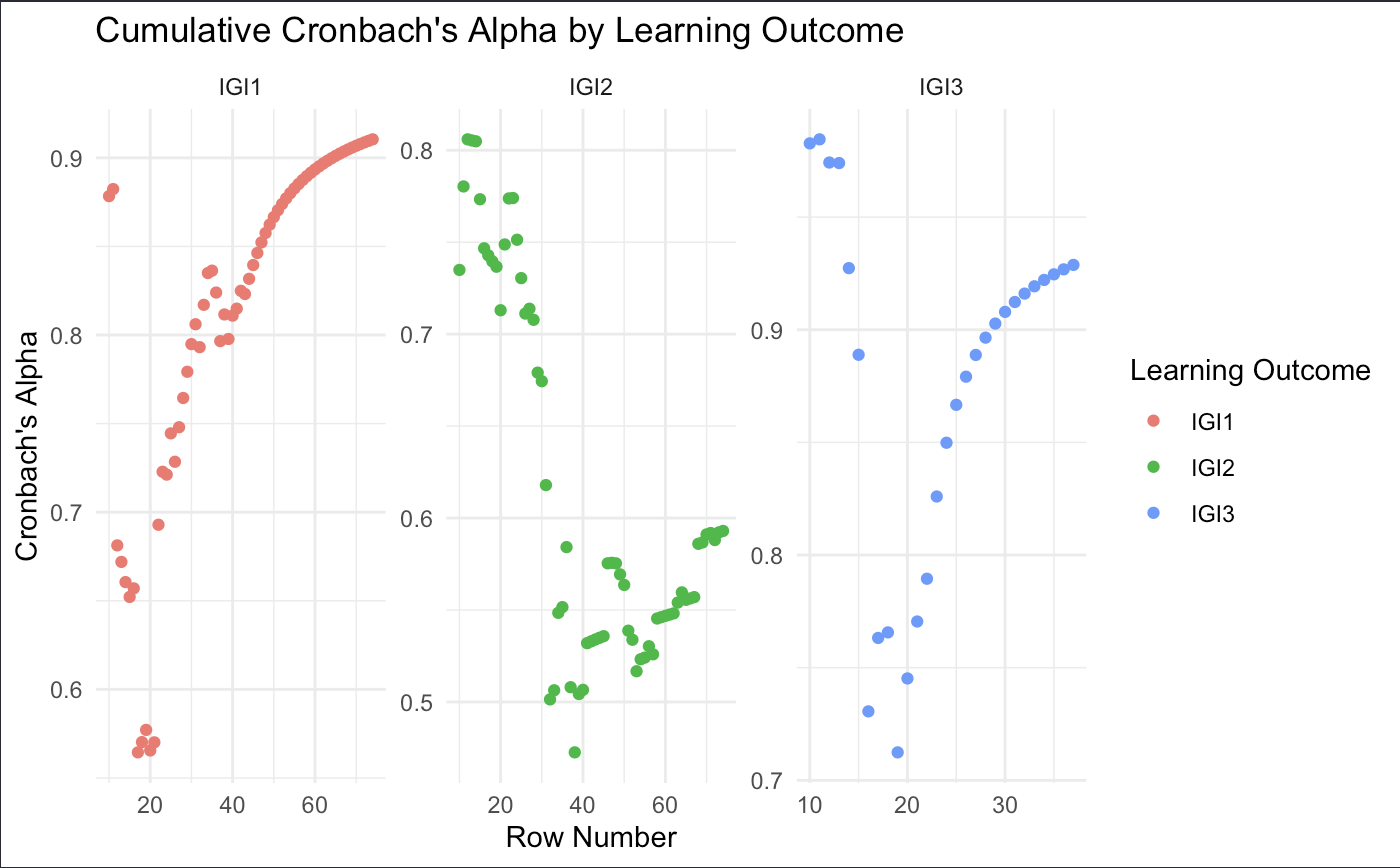
\includegraphics[width=1.0\textwidth]{visualizations/sub_sect_reliability.png}
    \caption{Here the three sub components of IGI are analyzed separately to see if one scoring component is more reliable than another. The fact that IGI 1 and IGI 3 reach above .8 reliability suggests that the lower reliability for IGI 2 is not due to rater training but due to the rubric itself.}
    \label{fig:sub_sect_reliability}
\end{figure}

To unpack these trends further, we conducted a fine-grained reliability analysis by sub-component, examining each rubric row within IGI1–3 independently. The results are shown in Figure~\ref{fig:fine_grained_reliability}. Here, the contrast becomes even clearer. While some sub-components (such as IGI1a/IGI1.1: reflection on personal worldviews) reached strong reliability, others (notably IGI2b/IGI2.2 and IGI3) showed persistent issues even in later batches. In particular, raters appeared to struggle with evaluating the influence of worldviews on perceptions of cultures and communities, and with the analysis of structural inequality. These categories may benefit from targeted rater training or further rubric clarification.

\begin{figure}[h]
    \centering
    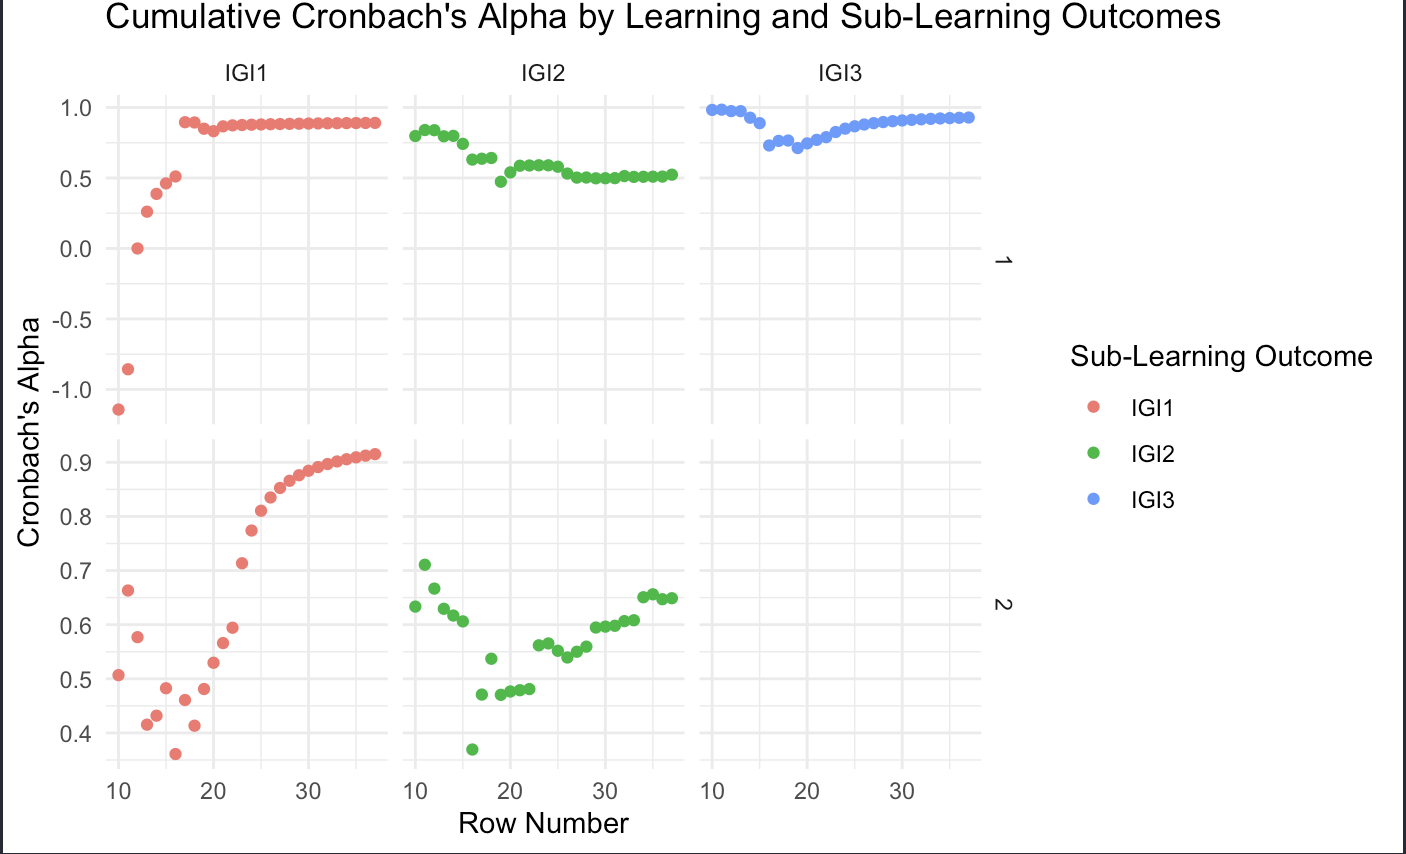
\includegraphics[width=1.0\textwidth]{visualizations/fine_grained_reliability.png}
    \caption{In this visual, the sub-components of the IGI rubric are tested for reliability separately. Here we can see that the main item with reliability issues is IGI 2 sub-component 2 (IGI2b). Reliability for all other sub-components is consistently high.}
    \label{fig:fine_grained_reliability}
\end{figure}

\subsection*{Discussion}

This multi-level analysis of rater agreement offers valuable insight into how rubric structure interacts with scoring consistency. The overall trend suggests that raters can and do calibrate over time, particularly when assignments are relatively stable and when learning outcomes are clearly defined. However, the sub-section and sub-component breakdowns make clear that some parts of the rubric remain more susceptible to interpretive variation. These findings highlight the need to treat reliability not as a binary outcome, but as a property distributed unevenly across an assessment instrument. Particularly, in the fine-grained reliability analysis, it becomes clear that IGI2 sub rubric question 2 (IGI2b) has much lower reliability. This finding is important to note as the reliability never goes above .6. While .6 inter-rater reliability is not terrible, the comparison to other reliability levels after the same amount of practice suggests that the other rubric questions elicit less variation between raters. That is, the IGI2 sub question 2 (IGI2b) may need to be reconsidered so that there is more reliability over time between raters. The variation currently suggests somewhat arbitrary rating between trained raters. 

Practically, this level of granularity allows assessment teams to move from generic statements of reliability to specific, actionable decisions about where to intervene. For instance, future calibration exercises might focus more attention on IGI2.2 (IGI2b) and IGI3, or reexamine how those criteria are operationalized in scoring rubrics. In addition, these results serve as a valuable baseline for AI model evaluation. If human agreement varies by rubric row, then alignment with AI outputs must also be considered at that level. Understanding the shape of human reliability is thus a prerequisite for interpreting the performance of AI-assisted scoring.

Taken together, these analyses validate the usefulness of the reliability script as a diagnostic tool —not just for validating current rater performance, but for identifying areas where targeted improvement is both possible and necessary within the rubric and for raters. They also reinforce the value of choosing IGI as a test case, given the richness of the rubric and the balance it strikes between structured guidance and open-ended interpretation.

\section{Background and Motivation for AI-Based Artifact Scoring}

As the scale and complexity of student assessment increase, educational institutions face mounting challenges in maintaining timely, consistent, and high-quality evaluation of student work. Human rating alone is labor-intensive, especially when artifacts are open-ended, span multiple disciplines, or target multiple learning outcomes. To address these challenges, we developed an AI-assisted artifact scoring workflow that leverages large language models (LLMs) to provide rubric-aligned evaluations of student work.

Unlike prior tools that focused only on rating infrastructure or inter-rater agreement, this system goes further by integrating a full pipeline—from preprocessing and prompt generation to model interaction and structured response storage. This approach allows the Dietrich assessment team to automate first-pass scoring, compare AI performance to human baselines, and iterate on workflows with far greater efficiency.

Figure~\ref{fig:strucutre_api} illustrates the scaffolded structure of the AI-assisted scoring system. At every step, the architecture treats the model not as a black-box oracle but as a rater—subject to the same constraints, structures, and documentation expectations as a human evaluator. Each artifact is linked to its instructional context, rubric criteria, and prompt set, enabling fine-grained tracking of input, output, and rationale. This modular structure supports not only scoring, but also auditing, training, and adaptation across different areas, assignments, and LLM models. It ensures that any new phase of testing—whether comparing models, refining prompts, or generating training examples—can be implemented cleanly within the same ecosystem. The core infrastructure is in place: what’s needed now is institutional support for continued training and refinement, building on a framework designed from the outset for transparency, accountability, and scale.

\begin{figure}[h]
    \centering
    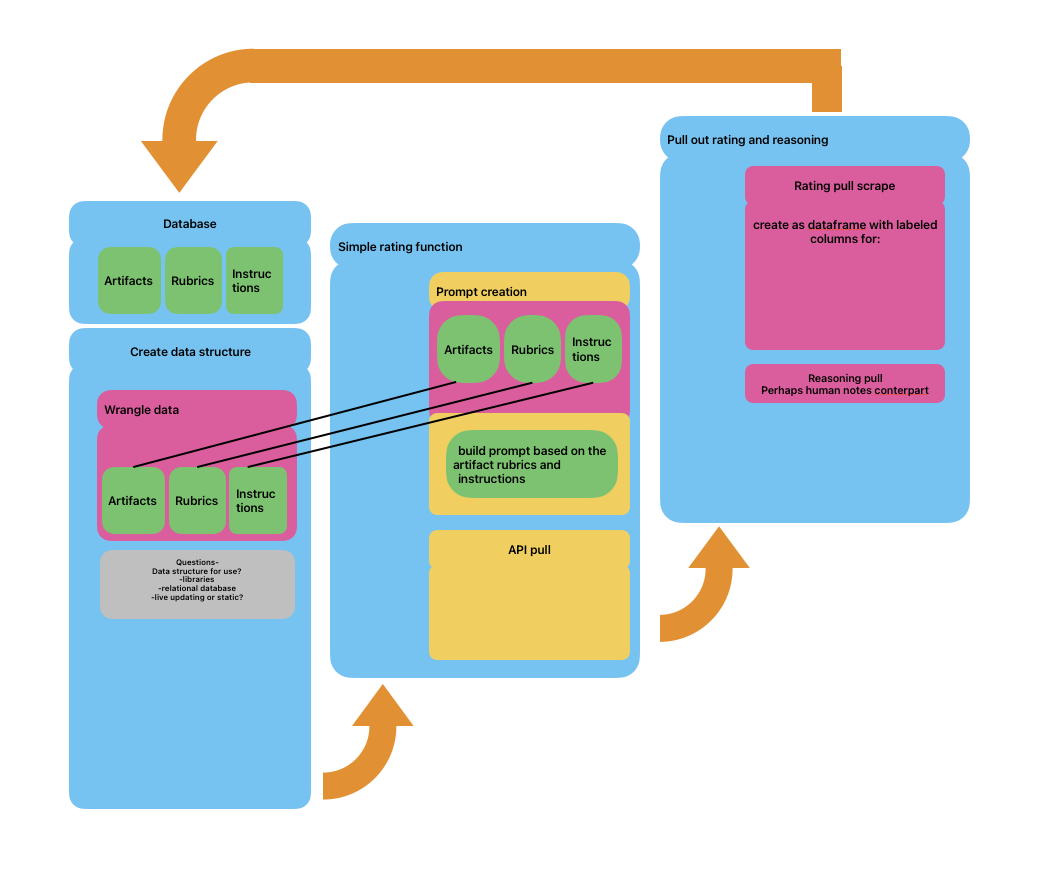
\includegraphics[width=1.0\textwidth]{visualizations/strucutre_api.png}
    \caption{This visual shows the basic strucutre of the artifact scoring pipeline for the LLM rating system.}
    \label{fig:strucutre_api}
\end{figure}

The goal is not to replace human judgment, but to augment it with fast, scalable support that align with institutional learning outcomes and complies with ethical and privacy requirements. This approach significantly reduces the overhead involved in artifact rating while laying the groundwork for longitudinal evaluation of model consistency, alignment with rubric structure, and reliability across assignment types. Examples of multiple scorings are listed in Appendix A as a sample for each IGI sub-component. 


\subsection*{Model Integration Strategy: Balancing Feasibility, Security, and Cost}

Selecting the right large language model (LLM) for automated artifact scoring involves more than choosing the most powerful model available. Especially in educational contexts, model selection requires balancing three critical factors: feasibility, security, and cost. This section outlines the rationale behind our decision to use GPT-4.0 mini, deployed through Carnegie Mellon University’s internal LiteLLM infrastructure.

\subsection*{Evaluation Criteria and Deployment Options}

During initial development, we considered several deployment routes, each with its own trade-offs. Public OpenAI APIs, while flexible and capable, retain user data unless an enterprise agreement is in place—rendering them incompatible with \href{https://studentprivacy.ed.gov/ferpa}{FERPA guidelines}. GitHub Copilot, although secure and inexpensive (this is secure for CMU use due to an enterprise agreement that CMU has made with Copilot-enterprise), is optimized for code and lacks the discourse awareness needed for rubric-based evaluation. Azure OpenAI and OpenAI Enterprise offer enterprise-grade security and flexibility but introduce high complexity (e.g., no API available or only for enterprises) and cost.

\subsection*{Final Model Selection: GPT-4.0 mini via CMU’s LiteLLM Deployment}

We ultimately selected GPT-4.0 mini, accessed through CMU’s LiteLLM proxy server. This choice reflects a deliberate effort to maximize output quality while minimizing both cost and administrative burden. GPT-4.0 mini strikes a practical balance—it is more capable than GPT-3.5 and significantly less expensive than full GPT-4, with response quality that aligns well with the needs of our rubric-based scoring system.

\subsubsection*{Feasibility}

GPT-4.0 mini handles Dietrich General Education artifacts without truncation and is fully compatible with our R-based prompt generation pipeline. Its outputs have proven to be rubric-sensitive, well-structured, and interpretable by faculty. The model supports both real-time scoring and batch processing, making it ideal for scalable assessment.

\subsubsection*{Security and FERPA Compliance}

All interactions with the model occur within CMU’s private infrastructure. No student data, prompts, or responses are transmitted to third-party servers. This setup guarantees FERPA compliance and protects the integrity of student submissions, while aligning with university data governance standards \cite{FERPA}. CMU’s LiteLLM proxy also provides access controls, usage tracking, and model switching functionality for future experiments.

\subsubsection*{Cost}

One of the strongest arguments for adopting GPT-4.0 mini is its cost efficiency. At a fraction of the price of full GPT-4 or Azure-based deployments, it enables large-scale scoring of thousands of artifacts at minimal expense. This affordability supports iterative development and prompt tuning without budgetary strain. Compared to full GPT-4, which can cost more than 25 times as much per artifact, GPT-4.0 mini offers a vastly more sustainable foundation for assessment.

\subsection*{Justification for Model selection}

The decision to deploy GPT-4.0 mini via CMU’s LiteLLM infrastructure reflects a thoughtful balance of pedagogical need, technical feasibility, data security, and institutional sustainability. This model offers a strong entry point into AI-assisted assessment, with performance that meets the demands of real scoring tasks, compliance with all student data regulations, and the ability to scale without compromising future growth. Crucially, the infrastructure supports easy model switching, allowing us to compare outputs from other models (e.g., full GPT-4 or domain-tuned variants) in subsequent phases of the project.

\subsection*{AI Reliability and Comparison to Human Raters}

To evaluate how reliable GPT-4.0 mini is under current deployment conditions, we conducted two sets of reliability comparisons using rubric-aligned scoring of IGI artifacts. The first analysis examined internal consistency of the model by prompting it multiple times with the same input, using fixed rubric structures. The second analysis compared AI outputs to human-generated scores, focusing on alignment across rubric dimensions and identifying points of divergence.

\subsection*{Agreement Across AI Runs}

Within-model consistency was measured by scoring each artifact multiple times using GPT-4.0 mini across 53 artifacts. Despite not being fine-tuned on local data or task-specific scoring conventions, the model performed relatively well. Across all rubric components, Kappa values ranged from 0.50 to 0.70. IGI1 subcomponents, which involve personal and others’ worldviews, showed strong internal consistency, with scores clustering near 0.66–0.70. IGI3, focused on structural inequality and institutional analysis, also scored well (around 0.68). IGI2 was more variable, with component 2.2 (which targets evaluation of cultural perspectives) dropping to 0.50—suggesting that more interpretive tasks generate less stable responses from the model.

Importantly, these reliability scores exceed those typically observed between human raters prior to training. In effect, the model enters the process at a more stable baseline than untrained human raters—an encouraging sign. But as we have seen in our human calibration data, consistency alone is not enough. What matters is alignment.


\subsection*{Agreement Between AI and Human Raters}

To evaluate alignment, we compared AI-generated scores with those assigned by trained human raters across 53 artifacts. Here, the model’s performance was weaker. Kappa scores ranged from 0.45 to 0.58 across rubric subcomponents, generally below the accepted threshold of 0.6. IGI1 components fared best again, with values in the 0.55–0.58 range, while IGI2.2 remained a problem area, hovering around 0.45. IGI3 scored at 0.56, showing only modest agreement with human ratings. Results can be seen in Figure \ref{fig:aivshuman}.

While these results fall short of the desired benchmark, they are meaningful. First, they indicate that the model is not fundamentally misaligned—many of its outputs are in the right general range. Second, they mirror the kinds of gaps we observed between human raters before structured calibration. Just as human raters needed training and discussion to converge on rubric expectations, so too does the model.

\begin{figure}[h]
    \centering
    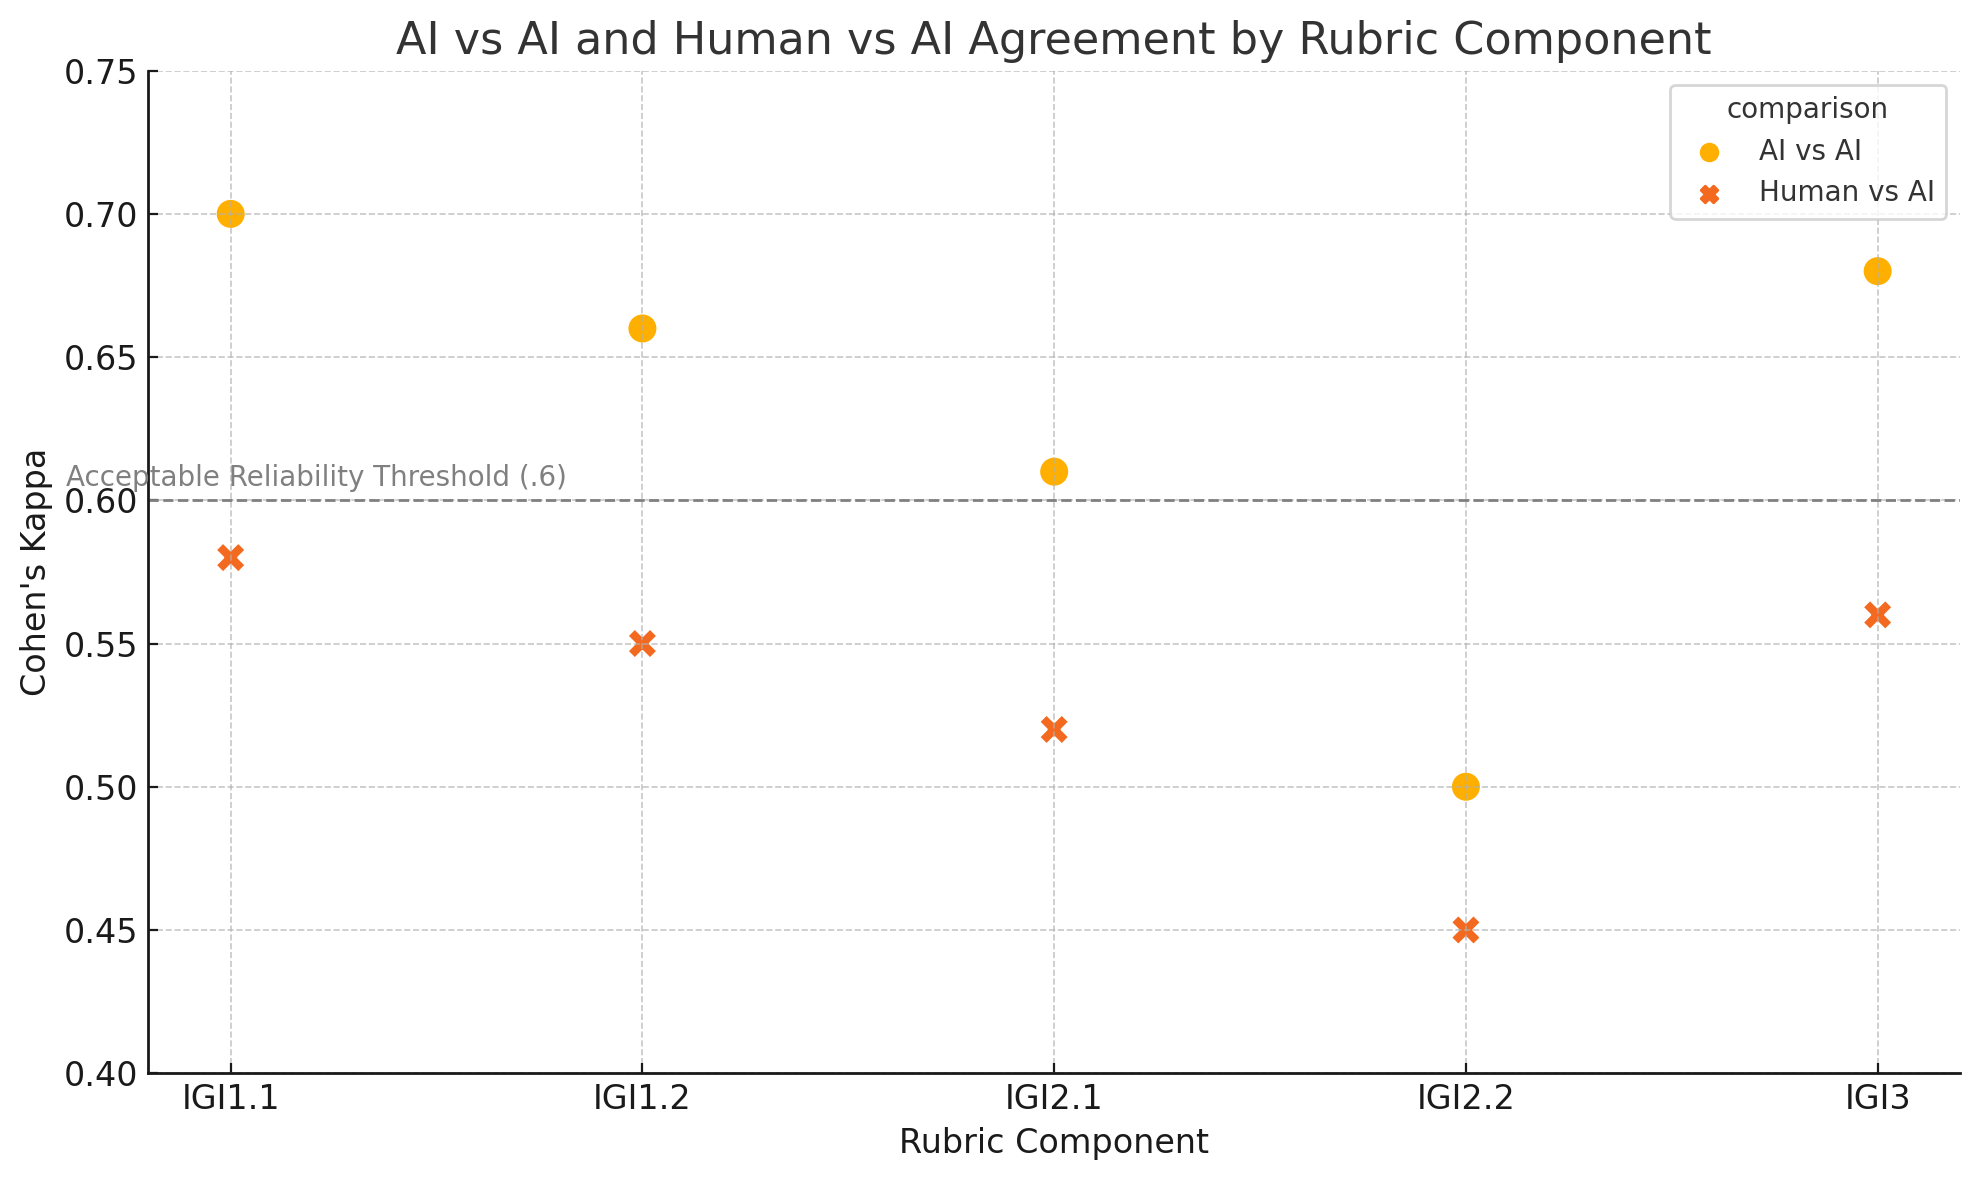
\includegraphics[width=1\textwidth]{visualizations/AI vs AI and Human vs AI Agreement by Rubric Component.png}
    \caption{Cohen's Kappa (reliability) values for each rubric subcomponent, comparing both within-AI reliability and AI vs. Human alignment. The dashed line at 0.6 reflects a commonly used reliability threshold. GPT-4.0 mini is more consistent than untrained human raters, but still falls short of alignment with trained human judgment—particularly in the more abstract subcomponents like IGI2.2(2b).}
    \label{fig:aivshuman}
\end{figure}

\subsection*{Takeaway}

The takeaway is clear: GPT-4.0 mini is consistent, interpretable, and promising—but untrained. Its performance out of the box rivals or exceeds that of untrained human scorers. But just like human raters, the model needs time, guidance, and tuning to reach production-level reliability. We now have the infrastructure and the results. What we need next is a dedicated semester of model comparison, prompt refinement, and domain-specific training to bring the system to full alignment.

\subsection*{Implications and Next Steps}

The results from this initial phase of testing reveal a compelling starting point: GPT-4.0 mini, as deployed within our system, is more internally consistent than untrained human raters. Across multiple rubric components, AI-to-AI agreement exceeds the levels of agreement observed between human raters prior to calibration. In that sense, the model is already operating at or above the baseline we expect from first-pass faculty scoring—an impressive result for an out-of-the-box system.

However, when compared to trained human raters—those who have participated in calibration sessions and received targeted feedback—GPT-4.0 mini still falls short. While human-human agreement improved over time through practice and clarification, the model received no such tuning. It was not trained on local rubrics, not exposed to exemplars, and not given any contextualized feedback about scoring logic. In this light, the performance gap is not a limitation of the model, but of the process.

Just as our raters improved over the course of the scoring cycle, so too can the model—if given the opportunity. What is needed now is not a new system, but a training phase: a structured semester dedicated to model comparison, targeted tuning, and alignment work. This training phase includes not only testing newer or larger models, but also investing in the existing system through prompt refinement, rubric-specific guidance, and integration of real faculty judgments. 

In effect, we now have an AI rater that is consistent, reliable, and FERPA-compliant—but undertrained. The infrastructure is in place. The proof of concept is complete. What’s needed next mirrors the investment we make in human raters: time, practice, and feedback. With that, GPT-4.0 mini—or whichever model proves most adaptable—can move from merely consistent to meaningfully aligned with the goals of our assessment process.

\subsection*{Concluding Thoughts on AI scoring}

This phase of development has delivered on its promise. We now have a working, cost-effective AI scoring infrastructure that supports secure, scalable, and interpretable evaluation of student artifacts. More importantly, we’ve shown that the system functions with a degree of consistency that rivals human judgment at baseline—and that it integrates cleanly into our existing assessment workflows.

But these results should not be misunderstood as an endpoint. They are a foundation. AI scoring systems, like human raters, require training. They require context. They require refinement. What we’ve built this year is a system that’s ready for that next step—one that doesn’t need to be redesigned, only deepened.

Moving forward, a dedicated semester of comparative evaluation, rubric alignment, and prompt tuning would allow us to complete what we’ve started. With continued support, the Dietrich College General Education Program will not only have a working model of AI-assisted scoring—it will have a validated, ethical, and scalable system ready for broader use. This is not just a technical achievement; it’s a roadmap for responsible innovation in higher education \cite{holmes2021AI, luckin2016AI}. And now is the time to follow it.

\section{Conclusion: Toward Sustainable, Transparent, and Scalable Assessment}

Over the past year, this fellowship has produced not only a set of functional tools but a foundational framework for modernizing educational assessment. The dynamic rating application replaced a fragmented and error-prone process with a secure, efficient system that centers user experience and data integrity. The reliability script added a layer of diagnostic insight—allowing for ongoing validation of both human and AI ratings. And the AI-assisted scoring pipeline established the infrastructure needed to scale these innovations in a cost-effective and FERPA-compliant way.

Together, these tools do more than solve isolated problems. They form a cohesive system that is modular, extensible, and ready for the next phase of integration. By treating both human and AI raters as participants in a shared evaluative structure, this work lays the groundwork for hybrid assessment models that are transparent, accountable, and pedagogically rigorous.

As we look ahead, the goal is not replacement—but refinement. Continued development will focus on model tuning, broader rubric coverage, and deeper comparisons across rating strategies. With institutional support and faculty collaboration, this system can evolve into a sustainable model of assessment that meets the demands of a changing educational landscape while upholding the standards of fairness, rigor, and insight that define effective evaluation.

This work marks not just a set of technical achievements, but a shift in how we think about assessment—less as a static task, and more as a dynamic, collaborative ecosystem. The tools are ready. The infrastructure is in place. Now is the time to build on this foundation.
\bibliography{sample}

\clearpage
\onecolumn
\appendix
\section*{Appendix A: Full Feedback Table Sample for each IGI Subcomponent of GPT output}


\begin{center}
\small
\renewcommand{\arraystretch}{1.2}
\begin{longtable}{|p{0.12\textwidth}|p{0.78\textwidth}|p{0.05\textwidth}|}
\caption{Formatted and wrapped feedback with scores for IGI learning outcomes.} \\
\hline
\textbf{Learning Outcome} & \textbf{Descriptive Feedback} & \textbf{Score} \\
\hline
\endfirsthead
\hline
\textbf{Learning Outcome} & \textbf{Descriptive Feedback} & \textbf{Score} \\
\hline
\endhead
IGI1.1 & \#\#\# **Response to Submission**\par Your research proposal on the beginner Chinese curriculum provides a comprehensive and thought-provoking exploration of the interplay between language learning and cultural contexts intrinsic to Chinese languaculture. Here's an evaluation of your work utilizing the rubric provided, along with suggestions for improvement:\par 1. **Research Questions**: \par    - Your research questions are clear and focused on the specific relationship between vocabulary, curriculum design, and cultural context. This clarity will aid in directing your study effectively.\par 2. **Rationale/Statement of Importance**: \par    - The rationale articulates well why understanding the languaculture behind language education is crucial. By linking linguistic fluency to cultural understanding, you underscore the practical implications of your research, which is excellent. However, to enhance this section, you might want to reflect more on how your personal experiences with language learning or teaching—particularly your own encounters with Chinese languaculture—have shaped your perspective on this issue.\par 3. **Proposed Data Collection Methods**: \par    - The methods outlined for data collection show a reasonable balance between quantitative and qualitative approaches. Conducting interviews with educators will undoubtedly enrich your findings. To deepen this, consider including reflections on how your own learning experiences influenced the questions you formulated for the interviews—this could align better with your personal worldview.\par 4. **Proposed Analytic Procedures**: \par    - Your proposed analysis seems robust, particularly in integrating qualitative insights from interviews with quantitative data from textbooks. However, it would benefit from a personal angle. How have your experiences as a language learner or educator shaped your understanding of what should be included in a beginner curriculum? Including your worldview here can give more context to your analytical framework.\par 5. **Statement of Possible Implications/Outcomes for Research and/or Practice**: \par    - This section summarizes potential contributions clearly. Emphasizing the real-world applications of your findings, such as curricular development and teaching methodologies, shows how your project is not solely theoretical. Highlighting how cultural contexts from your personal experience inform these implications would enhance your connection to the research outcomes.\par \#\#\# **Personal Worldview Reflection**\par To align your proposal more closely with the rubric, I encourage you to incorporate specific narratives or experiences that have shaped your understanding of language learning amidst cultural contexts. For instance, reflecting on any challenges you faced when learning Mandarin could enrich the proposal. Did you notice discrepancies between what you learned and colloquial usage? Did interactions with native speakers provide insights into the languaculture that formal education overlooked? By integrating such reflections, you would not only clarify your personal worldview but also establish a richer context for your research.\par \#\#\# **Scoring Level Recommendation**\par Given this evaluation, I would place your proposal at Level 2.0 in the rubric because while you present an interesting and relevant study, the personal worldview component is somewhat underdeveloped. By weaving in your personal narrative and cultural influences more explicitly, you can elevate your score to Level 3.0 or higher, creating a more engaging and comprehensive proposal.\par **Overall, you have a strong foundation. With these enhancements, your project can reflect not only the academic rigour of your research but also the personal insights that truly make learning a comprehensive journey.** & 2 \\
\hline
IGI1.2 & Your research proposal on the "Beginner Chinese Curriculum" demonstrates a thoughtful approach to the intersection of language and culture. Below is a reflective response based on the rubric provided:\par \#\#\# Reflection on Personal Worldview\par Through this research proposal, I recognize that my personal worldview has been shaped significantly by my experiences with language learning and cultural immersion. Growing up in a multicultural environment, I was always aware of the nuances in language that extend far beyond vocabulary, including the cultural contexts that inform how language is used in everyday life. My experiences have led me to value not just words, but the meanings, histories, and sentiments that accompany them, which seem integral to achieving fluency. \par \#\#\#\# Acknowledgment of Cultural Contexts\par The proposal reflects the belief that language learning is incomplete without understanding the cultural underpinnings—what I would refer to as "languaculture." This perspective stems from my own challenges in learning languages that often do not directly translate phrases or concepts due to cultural differences. For instance, early on in my language studies, I struggled with idiomatic expressions in Mandarin that lacked direct English counterparts. This highlighted for me the necessity of integrating cultural education alongside linguistic skill development.\par Moreover, working with diverse groups of learners, I have observed how cultural contexts impact motivations, learning styles, and ultimately, language acquisition. My interactions with educators and students from various backgrounds have confirmed that successful language education must consider the cultural values and practical applications within daily conversations. In proposing an analysis of vocabulary sets in beginner curriculums, I aim to advocate for an approach that closely aligns with how native speakers truly converse, thereby bridging the gap between language education and cultural competency.\par \#\#\#\# Synthesizing Insights and Acknowledging Limitations\par In synthesizing these insights, I aim to highlight the disconnection between educational materials and colloquial language use, as articulated in the proposal. This gap has real implications for language learners who, like me, seek to use their skills in meaningful ways. At the same time, I acknowledge the limitations of my perspective. Different learners may prioritize different aspects of language learning—some may find value in structured vocabulary and traditional curriculums, while others may thrive in immersive, culturally rich environments. \par Ultimately, this nuanced understanding of my personal worldview serves as a foundation for my research. It drives my inquiry into how beginner Chinese curriculums can evolve to reflect the realities of Chinese languaculture, fostering better communication and cultural understanding for learners at all levels.\par \#\#\# Score Assessment\par Given the depth of reflection and the acknowledgment of cultural contexts in shaping my personal worldview, I believe this response aligns with **Level 4.0** on the rubric. It comprehensively explains my personal experiences and insights while integrating multiple cultural contexts and acknowledging potential limitations, ensuring a well-rounded perspective on the subject matter. \par ---\par By revisiting this proposal with clearer reflections of how my cultural background has influenced my approach, I hope to create a richer dialogue on the importance of integrating culture into language education. If there are specific areas where you would like me to expand further or if you have additional questions on this topic, please let me know! & 4 \\
\hline
IGI2.1 & \#\#\# Response to Beginner Chinese Curriculum Research Proposal\par Your proposal on designing a study to investigate beginner Chinese language curriculums through the lens of languaculture is incredibly well-structured and insightful. Below, I will address specific elements of your project and provide suggestions for enhancing clarity and depth.\par 1. **Research Questions**: Your questions are relevant and clearly articulated. They establish a foundation for exploring the intersection of language and culture within the context of teaching Mandarin. It might be beneficial to expand on how you will define "value" in terms of educators’ perspectives on vocabulary. This could help target more specific cultural practices or beliefs influencing curriculum choices.\par 2. **Rationale/Statement of Importance**: You effectively highlight the gap in current curriculums and the importance of culturally relevant vocabulary for language learners. To strengthen this, consider including personal insights or any specific experiences that led you to this topic. For instance, if you encountered difficulties when learning Mandarin due to cultural discrepancies in vocabulary, sharing such experiences could enhance your argument and provide a personal connection to the research.\par 3. **Proposed Data Collection Methods**: Your methods are both comprehensive and practical. In addition to analyzing textbooks and conducting interviews, you might consider incorporating participant observations in language classrooms or language exchange groups. This could provide observational data on how vocabulary is utilized by learners in real-time situations, adding another dimension to your analysis.\par 4. **Proposed Analytic Procedures**: The combination of quantitative and qualitative analysis is a well-thought-out approach. It might be helpful to clarify how you will display your findings. For example, will you use tables, charts, or narrative descriptions? Additionally, discussing potential coding strategies for qualitative data could demonstrate a deeper understanding of how to analyze interview responses related to languaculture.\par 5. **Possible Implications/Outcomes**: You anticipate practical applications for your research, which is essential for its potential impact. It may be useful to discuss who specifically could benefit from your findings—such as educators, curriculum developers, or even students. Acknowledging any limitations of your study (such as the variability in learners' cultural backgrounds or differing regional usages of Mandarin) could also provide more nuance to your conclusions.\par \#\#\# Personal Reflection and Cultural Context\par In reflecting on your proposal, it’s evident that your approach stems from a culturally conscious perspective, highlighting the significance of languaculture in language education. To achieve a higher score on the rubric, consider synthesizing multiple cultural contexts that have shaped your own understanding of language learning. For example, how has your background, experiences in language acquisition, or interactions with native speakers influenced your views on curriculum design? Acknowledging these aspects could provide a more comprehensive explanation of your personal worldview while connecting to broader themes in language education.\par In summary, your proposal is already strong, and incorporating personal elements along with enhanced clarity in your methods and analyses could further strengthen it. I look forward to seeing how you develop these ideas in your final submission. & 2 \\
\hline
IGI2.2 & Thank you for sharing your research proposal on the Beginner Chinese Curriculum and how it reflects Chinese languaculture. Here’s a thoughtful response:\par \#\#\# **Reflection on Proposal**\par Your proposal presents a significant and timely investigation that addresses a real gap in current language education methodologies, particularly for learners of Mandarin. Your research questions focus on how Chinese language educators value different types of beginner vocabulary sets and their impact on understanding the broader concepts of Chinese languaculture. This is particularly relevant given the increasing global interest in Mandarin as a second language.\par \#\#\# **Cultural Contexts and Personal Worldview**\par 1. **Understanding Personal Connection**:\par    It's apparent that your interest in this topic might stem from your personal experiences with language learning or exposure to Chinese culture. Reflecting on your own journey in learning Mandarin, whether it was through formal education or interaction with native speakers, can further enrich your research. For instance, how did your own understanding of Chinese culture influence your approach to learning the language? Were there specific cultural elements or societal nuances you encountered that shaped your perception and fluency in Mandarin?\par 2. **Acknowledging Cultural Contexts**:\par    The proposal hints at personal stakes in the methodology of teaching language to non-native speakers. By exploring how various vocabulary sets are used in different contexts, you're implicitly recognizing the influence of cultural norms on language learning. This points to an understanding that language is not simply a set of grammatical rules but is deeply intertwined with cultural practices and values. Sharing specific examples from your own language-learning experiences can enhance this acknowledgment. For instance, were there moments in your learning when colloquial phrases differed greatly from textbook vocabulary, and how did that impact your fluency or understanding of everyday interactions?\par 3. **Synthesis of Cultural Influences**:\par    To reach the highest scoring level, consider delving deeper into how multiple cultural contexts inform your view of education, language acquisition, and communication. This could include the influence of Western educational philosophies versus Eastern ones, and how these might impact curriculum design. Additionally, reflecting on societal attitudes toward language learning in different settings can provide a broader perspective. Were your learning experiences informed by cultural narratives that typically favor certain types of communication over others?\par 4. **Limitations and Future Directions**:\par    Acknowledging the limitations of your own experiences and perspectives can offer a balanced view. What assumptions might you bring to your research based on your cultural background? How do these potential biases inform your understanding of what constitutes 'effective' vocabulary in language learning? By addressing these aspects, you demonstrate a thoughtful awareness of the complexity of cultural influences on both education and personal identity.\par \#\#\# **Conclusion**\par Overall, your research proposal demonstrates a clear and relevant focus on improving Chinese language education through an understanding of culturals nuances. However, enriching your analysis with reflections on your personal experiences and addressing the interrelatedness of multiple cultural contexts will create a more comprehensive narrative. By doing so, you'll not only strengthen your proposal but also enhance your understanding of how these cultural contexts shape both curriculum and personal identity in language learning.\par In summary, your exploration of languaculture, specifically in the context of Mandarin language education, has the potential to bridge gaps in understanding and provide practical benefits for future learners. By being reflective about your own viewpoint and acknowledging broader cultural influences, you can ensure a nuanced approach to your research.\par \#\#\# Questions for Further Thought:\par - How did your background inform your initial perspectives on learning Mandarin?\par - What experiences did you have with cultural misunderstandings while learning the language? How did those shape your understanding of language as a social tool?\par - In what ways do you think language education can better incorporate cultural elements that resonate with learners' personal experiences?\par This reflective framework can be beneficial as you continue to develop your research proposal. Good luck with your project, and I look forward to seeing where you take it! & 3 \\
\hline
IGI3.1 & \#\#\# Response to Languaculture Research Proposal\par Your proposal on investigating the relationship between beginner Chinese vocabulary education and Chinese languaculture is comprehensive and insightful. Here are my reflections and considerations based on the rubric provided.\par 1. **Research Questions**: Your research questions are well-defined and relevant to the interplay of language and culture. By examining how educators value vocabulary and how this reflects larger cultural ideologies, you position your research within a significant area of inquiry. \par 2. **Rationale/Statement of Importance**: You effectively articulate the significance of your study, discussing the gap in current curriculums related to cultural context and fluency. However, to enhance your rationale, you might consider including a personal anecdote about your own experiences learning Chinese or observing these cultural discrepancies. This could provide a more robust connection to your personal worldview and highlight the importance of your research on a more personal level.\par 3. **Data Collection Methods**: Your proposed methods for data collection are thorough and well-structured. The comparative analysis of educational texts and native literature will provide a rich basis for understanding the discrepancies in vocabulary. Additionally, the interviews with curriculum creators are a strong method to gain qualitative insights. It might be useful to include how you plan to recruit these educators for interviews and ensure a diverse representation of perspectives.\par 4. **Analytic Procedures**: You clearly outline a mixed-methods approach that combines quantitative and qualitative analysis, which is essential for understanding the complexities of languaculture. As you plan your analysis, consider discussing potential limitations in your data, such as the bias in selecting materials or the linguistic variations in different regions of China, which could influence vocabulary use.\par 5. **Implications/Outcomes**: Your proposed outcomes center around improving language education and understanding the values embedded in Chinese culture, which is commendable. To strengthen this section, you might explore how the findings could affect specific groups (e.g., educators, curriculum developers, students) and the broader implications for intercultural communication.\par **Personal Worldview Reflection**: In considering the scoring criteria, I see an opportunity for you to enhance your response to Level 4. To align with this scoring, you could synthesize multiple cultural contexts that have influenced your understanding of language learning, such as your background, the culture of your language instructors, and the significant cultural elements of China itself. Acknowledging how these contexts shape your views on effective language education and fluency could enrich your proposal and connect your research more personally.\par Overall, your proposal is compelling and thoughtfully designed, contributing to the understanding of languaculture in language education. Further personal reflections linked to cultural contexts could elevate the depth of your discussion and align more closely with the expectations set by the rubric. I encourage you to incorporate these suggestions as you refine your proposal. & 2 \\
\hline
\end{longtable}
\end{center}


\twocolumn

%\twocolumn

\end{document}